\chapter{\implementationdevelopmentname}\label{chp:implementacion}

En esta sección se presenta detalladamente la implementación del algoritmo desarrollado para abordar el objetivo de este trabajo, sus atributos y su evolución hasta llegar a la solución final.

\section{Elección de la Técnica de Optimización}

Como se ha visto en el apartado del estado del arte, los problemas de optimización se pueden abordar con diferentes técnicas dependiendo de las características del problema.

Una de las técnicas que ofrece soluciones óptimas, a costa de un gran tiempo de cómputo, es la programación lineal entera (ILP). El estudio \textit{Networking for a Low-Carbon Future: An ILP-Based Carbon-Aware Approach for SDN} \cite{GomezdelaHiz2025} muestra cómo esta técnica es capaz de reducir las emisiones de carbono en hasta un 84.5\%, aunque el tiempo de ejecución llegó a alcanzar los 17 minutos, lo que es prohibitivo en escenarios tan cambiantes. 

Como alternativa a soluciones basadas en ILP, se pueden usar técnicas de \textit{Deep Learning} (DL). Pero estas técnicas, además de requerir una gran cantidad de datos para entrenar el modelo, no son viables para este tipo de problemas, pues en el momento en el que se modifique la topología de red, el modelo entrenado dejará de ser válido, lo que obligará a volver a entrenar el modelo desde cero, con la consecuente pérdida de tiempo y recursos.

Los algoritmos genéticos pueden ser una buena opción, pero suelen requerir una considerable cantidad de tiempo de ejecución, especialmente para problemas con un gran espacio de búsqueda. Al estar tratando con un escenario en el que el tiempo es crítico, pues las necesidades de la red cambian a lo largo del día, las soluciones basadas en algoritmos genéticos no son factibles.

Por otro lado, los algoritmos voraces son rápidos y fáciles de implementar. Estas soluciones eliminan la problemática de los tiempos de ejecución largos que presentan las técnicas anteriores. Sin embargo, toman decisiones basadas únicamente en la información local sin considerar el impacto a largo plazo. Esto puede llevar a soluciones subóptimas o, incluso, a soluciones inviables si se toman decisiones que comprometen la conectividad de la red. Realmente, que un algoritmo voraz encuentre una solución subóptima no es algo inherentemente malo, pues ya se estaría hablando de una mejora significativa respecto a la situación inicial, pero el hecho de que pueda encontrar soluciones inviables es un riesgo que bajo ningún concepto se puede permitir.

En cambio, las soluciones basadas en PSO son una gran opción para este tipo de problemas, ya que son capaces de explorar el espacio de búsqueda de manera eficiente y encontrar soluciones, aunque no sean óptimas, en un tiempo razonable. Respecto a los algoritmos voraces, PSO ofrece la ventaja de ofrecer siempre soluciones factibles. Además, como PSO es un algoritmo de optimización global, tiene la capacidad de evitar caer en óptimos locales. Teniendo en cuenta que se tratan de problemas con grandes espacios de búsqueda, es fundamental evitar a toda costa los óptimos locales.

Otra ventaja de PSO es que existen numerosas implementaciones disponibles, lo que facilita su uso y permite centrarse en la modelización de la función objetivo. Además, PSO es un algoritmo relativamente sencillo de ajustar, con pocos parámetros a configurar, facilita la realización de barridos para encontrar la configuración que mejor se adapte al problema en cuestión.

Es por esto que se ha optado por usar PSO como técnica de optimización para abordar el problema de optimización de las emisiones de $CO_2$ en redes cableadas.

\section{\textit{Particle Swarm Optimization}}\label{sec:pso}

Como en la mayoría de algoritmos de optimización evolutivos, PSO se basa en la idea de iterar sobre un conjunto de soluciones candidatas, partículas, y actualizar estas soluciones en función de su rendimiento.

\begin{figure}[H]
\centering
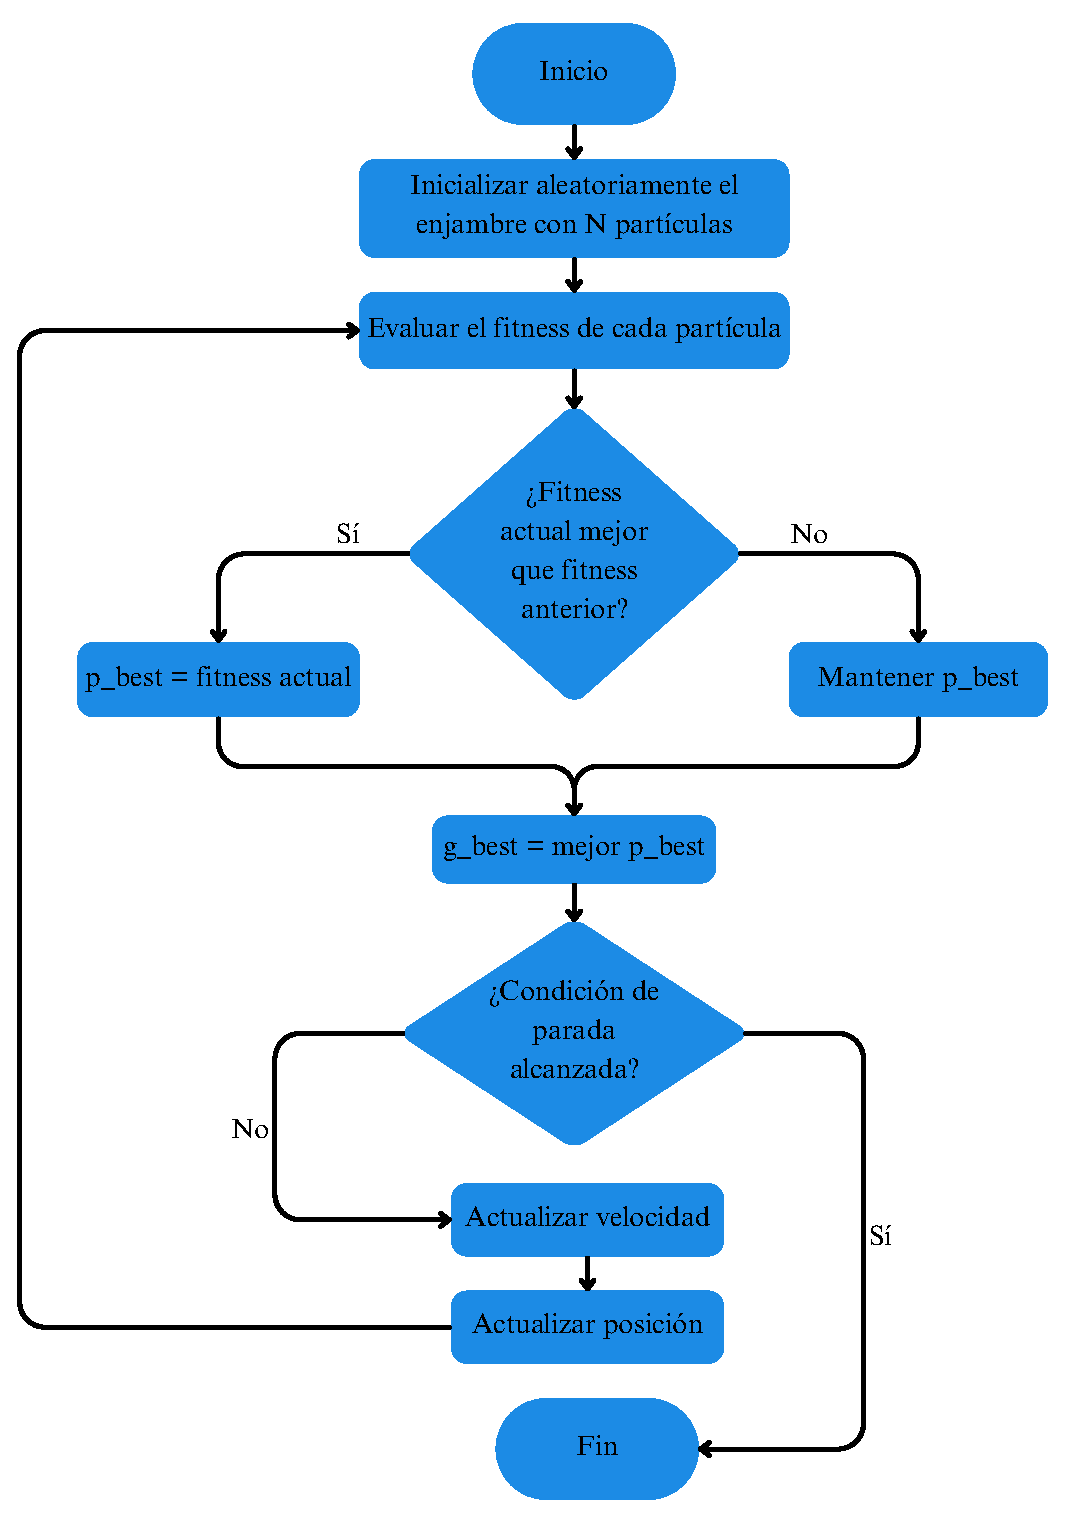
\includegraphics[width=0.6\textwidth]{pictures/pso_flowchart.pdf}
\caption[Diagrama de flujo de PSO]{Diagrama de flujo de PSO.\\Fuente: Elaboración propia.}
\label{fig:pso_flowchart}
\end{figure}

Para entender mejor el diagrama de flujo que se muestra en la \autoref{fig:pso_flowchart}, se va a usar un sencillo ejemplo: personas buscando una localización en un mapa.

\begin{enumerate}
    \item PSO inicializa aleatoriamente el enjambre con un número determinado de partículas, que traducido al ejemplo, sería posicionar a las personas en el mapa de manera aleatoria.
    \item Luego, cada persona evalúa la calidad de su posición (cada partícula evalúa el fitness), es decir, cómo de cerca está de la localización objetivo.
    \item A continuación, cada persona compara su posición actual con la mejor posición que ha encontrado hasta ese momento (p\_best) y, en caso de ser superior, actualiza su mejor posición personal.
    \item Después, los individuos se comunican entre sí para compartir información sobre sus mejores posiciones personales, lo que les permite conocer la mejor posición global encontrada por el grupo (g\_best).
    \item Si se ha alcanzado la condición de parada, como puede ser un número máximo de intentos, el grupo comunica la mejor posición global encontrada, que sería la localización más cercana al objetivo. Si no se ha alcanzado la condición de parada, cada persona, en función de la información recabada hasta el momento, se mueve a otra posición (actualizar velocidad y actualizar posición) y se vuelve a evaluar la calidad de su nueva posición, empezando así una nueva iteración.
\end{enumerate}

\section{Parámetros de PSO}

En esta sección se detallan los parámetros que influyen en la ejecución de PSO, como pueden ser las partículas, el coeficiente de inercia, el coeficiente cognitivo, el coeficiente social, el número de vecinos y las dimensiones del espacio de búsqueda. Cada uno de estos parámetros tiene un impacto significativo en el rendimiento del algoritmo y en la calidad de las soluciones encontradas, por lo que es importante entender su función y cómo afectan al comportamiento del algoritmo.

\subsection{Partícula}

El concepto de partícula ya se ha comentado brevemente con anterioridad, y es que una partícula es un agente individual que representa una solución candidata al problema de optimización. Como se ha comentado en el ejemplo anterior, se puede entender por partícula a una persona buscando la ubicación objetivo del mapa. De hecho, este ejemplo no se aleja mucho de la inspiración original de PSO, puesto que se basa en el comportamiento social de bandadas de pájaros o bancos de peces moviéndose en grupo hacia un objetivo común.

%Dado que PSO es un algoritmo inspirado en el comportamiento social de los animales, como las bandadas de pájaros o los bancos de peces, se puede imaginar cada partícula como un pájaro que está sobrevolando el terreno, el espacio de búsqueda, en busca de la zona con más comida, la mejor solución.

\subsection{Función objetivo}

La función objetivo es una parte fundamental de cualquier algoritmo de optimización, pues se trata de la función que se usa para evaluar cada solución candidata y determinar qué tan buena es esa solución. En el caso de PSO, la función objetivo se utiliza para evaluar la calidad de cada partícula en cada iteración, y se utiliza para actualizar la mejor posición personal de cada partícula y la mejor posición global del enjambre.

\subsection{Velocidad}

En PSO, las partículas tienen dos atributos principales, siendo la velocidad uno de ellos. Esta determina en qué dirección y cuánto se mueve cada partícula a lo largo del espacio de búsqueda. La velocidad se actualiza en cada iteración en función de la mejor posición personal de la partícula y la mejor posición global del enjambre, lo que permite que las partículas exploren el espacio de búsqueda de manera eficiente. Una velocidad alta puede permitir que las partículas exploren el espacio de búsqueda de manera más amplia, pero también puede hacer que el algoritmo sea más propenso a saltar sobre buenas soluciones. Por otro lado, una velocidad baja puede hacer que el algoritmo sea más lento, pero también puede ayudar a que las partículas se concentren en áreas prometedoras del espacio de búsqueda.

\subsection{Posición}

El segundo atributo principal de las partículas es la posición, que representa una posible solución al problema de optimización. La diferencia entre la posición y la partícula, pues las definiciones pueden ser un poco confusas, es que la posición es el valor actual de la solución representada por la partícula, mientras que la partícula es el agente que se mueve a lo largo del espacio de búsqueda. Siguiendo con el ejemplo de las personas y el mapa, la posición sería el lugar específico donde se encuentra un individuo en un momento dado. La posición se actualiza en cada iteración en función de la velocidad de la partícula, lo que permite que las partículas se muevan a través del espacio de búsqueda y encuentre mejores soluciones.

\subsection{Coeficiente de inercia}

El coeficiente de inercia es un parámetro que controla la influencia de la velocidad anterior en la actualización de la velocidad actual de cada partícula. Un coeficiente de inercia alto hace que las partículas mantengan su velocidad anterior, lo que puede ayudar a que el algoritmo explore el espacio de búsqueda de manera más amplia. Por otro lado, un coeficiente de inercia bajo hace que las partículas sean más propensas a cambiar su velocidad en función de la mejor posición personal y global, lo que puede ayudar a que el algoritmo se concentre en áreas prometedoras. Es importante encontrar un valor adecuado para este parámetro en función del problema específico, ya que un valor demasiado alto o demasiado bajo puede afectar negativamente al rendimiento del algoritmo.

\subsection{Coeficiente cognitivo}

El coeficiente cognitivo es un parámetro que controla la influencia de la mejor posición personal de cada partícula en la actualización de su velocidad. Un coeficiente cognitivo alto hace que las partículas se centren más en su propia experiencia, lo que ayuda a que el algoritmo se centre en áreas prometedoras. Por otro lado, un coeficiente cognitivo bajo hace que las partículas sean más propensas a seguir la mejor posición global del enjambre, lo que puede ayudar a que el algoritmo explore el espacio de búsqueda más ampliamente.

\subsection{Coeficiente social}

El coeficiente social es un parámetro que controla la influencia de la mejor posición global del enjambre en la actualización de la velocidad de cada partícula. Un coeficiente social alto hace que las partículas se centren más en la experiencia colectiva del enjambre, lo que puede ayudar a que el algoritmo explore el espacio de búsqueda más ampliamente. Por otro lado, un coeficiente social bajo hace que las partículas sean más propensas a centrarse en su propia experiencia, así el algoritmo se concentra en áreas prometedoras. Es importante encontrar un equilibrio adecuado entre el coeficiente cognitivo y social, ya que un desequilibrio puede desembocar en soluciones subóptimas.

\subsection{Número de vecinos}

Este parámetro controla la cantidad de partículas que se consideran como vecinos de cada partícula en la actualización de su velocidad. Si el número de vecinos es alto, cada partícula se ve influenciada por un gran número de otras partículas, lo cual hace que se centre más en la experiencia colectiva del enjambre. En cambio, si el número de vecinos es bajo, cada partícula se ve influenciada por un número reducido de otras partículas, centrándose más en su propia experiencia. 

\subsection{Dimensiones del espacio de búsqueda}

Este parámetro define el número de dimensiones que tiene el espacio de búsqueda, lo que a su vez determina la cantidad de variables que se están optimizando. Por lo general, cuantas más dimensiones tenga el espacio de búsqueda, más complejo será el problema de optimización, ya que habrá más variables a considerar, pero puede permitir encontrar mejores soluciones. Por el contrario, un espacio de búsqueda con pocas dimensiones puede ser más fácil de explorar, pero también puede limitar la calidad de las soluciones encontradas. 

\section{Aproximación al Problema}

Con los conceptos básicos de PSO ya explicados, es importante entender cómo se ha aplicado este algoritmo al problema específico de optimización de las emisiones de $CO_2$ en redes SDN.

La primera solución que se planteó fue tranformar el espacio discreto del problema en un espacio continuo, lo que permitiría usar PSO en su forma original. Sin embargo, esta aproximación terminó descartándose, pues la umbralización hacía que PSO trabajase a ciegas. Es decir, no era capaz de discernir entre los cambios que se producían por debajo del umbral, lo que se considera como un enlace apagado, por tanto PSO no sabía si esos cambios apuntaban a una mejora o a un empeoramiento de la solución, lo que generaba un comportamiento errático del algoritmo.

\begin{figure}[H]
\centering
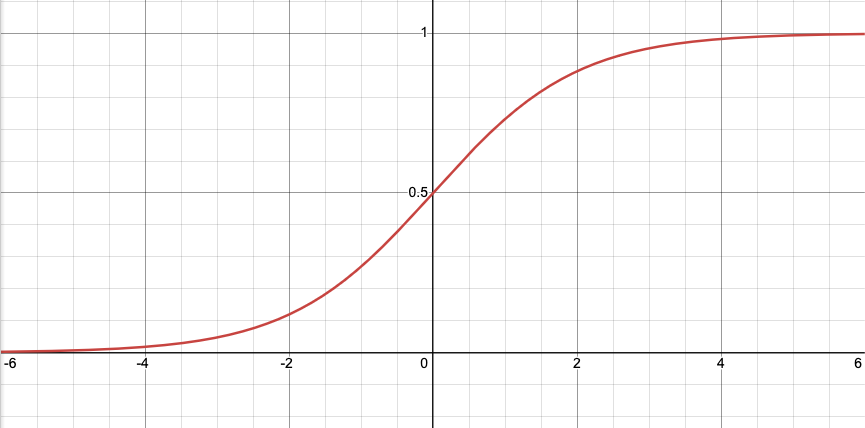
\includegraphics[width=0.6\textwidth]{pictures/sigmoide.png}
\caption[Función sigmoide]{Representación gráfica de la función sigmoide.\\Fuente: Elaboración propia.}
\label{fig:sigmoide}
\end{figure}

Más adelante, se iteró sobre la idea anterior de transformar el espacio discreto en continuo, pero esta vez usando una función sigmoide para umbralizar a través del cálculo de la probabilidad de que un enlace esté activo o apagado. Sin embargo, y como se muestra en la \autoref{fig:sigmoide}, se observó que, a medida que el valor continuo de la partícula, $x$, se aleja del cero, la curva se vuelve casi plana. Esto hace que, si el algoritmo decide que el enlace debe estar encendido, la velocidad de PSO empuje el valor de $x$ hacia números positivos cada vez más altos. Pero si más tarde el algoritmo decide que ese enlace en realidad debe estar apagado, PSO tardará muchas iteraciones en generar una velocidad lo suficientemente negativa como para arrastrar el valor de $x$ de vuelta al cero. En todo ese tiempo, la partícula está estancada y pierde capacidad de exploración.

Finalmente, se optó por hacer uso de adaptaciones de PSO para espacios de búsqueda discretos. De esta manera, se evitan los problemas de "cegera" de la umbralización y las pérdidas de capacidad de exploración que se observaban con la función sigmoide. Además, esto permite que PSO trabaje directamente con el espacio discreto del problema, mejorando así la eficiencia del algoritmo.

En el entorno de las redes SDN, la solución propuesta se implementaría en el controlador SDN, lo que permitiría a PSO tener acceso a información en tiempo real sobre el estado de la red y evaluar a lo largo del día los cambios que habría que hacer en cada momento para mantener las emisiones de $CO_2$ al mínimo.

\subsection{Estrategias de manejo de restricciones}

Para que el algoritmo sea realmente efectivo, se han de tener en cuenta las restricciones estrictas de la red, como pueden ser asegurar la conectividad total o no sobrepasar el ancho de banda. Para ello, se han evaluado dos aproximaciones de la función objetivo: PSO con penalización estricta y PSO con manejo de violación de restricciones.

\subsubsection{PSO con penalización estricta}

En esta variante, cuando una partícula propone una configuración de red que viola cualquiera de las restricciones, la función objetivo devuelve el valor infinito. En otras palabras, la posición de la partícula sufre una "muerte súbita", pues corta de golpe en el momento en el que no cumple una restricción.

La ventaja principal que presenta esta estrategia es la rapidez, pues el algoritmo descarta de manera inmediata una solución que no cumple con alguna restricción. Pero esta rapidez computacional le genera "ceguera" a PSO al no ser capaz de saber cuán buena es una solución inválida.

\subsubsection{PSO con manejo de violación de restricciones}

A diferencia de la variante anterior, el método \textit{Violation Constraint Handling} (VCH) no descarta una solución de manera inmediata, sino que contabiliza la cantidad de veces que se ha violado alguna restricción ($v$) y la multiplica por un factor de penalización ($P$). Este valor se suma a las emisiones de $CO_2$:

\begin{equation}
    f_{fitness} = f_{emisiones} + v \cdot P
\end{equation}

Este manejo más controlado de las violaciones proporciona a PSO un gradiente de información. De esta manera se puede discernir si una solución es menos mala que otra, lo que permite a las partículas atravesar zonas de inviabilidad para alcanzar regiones óptimas. Aunque es más lento que la versión anterior, puesto que el algoritmo debe realizar todos los cálculos para cada posición de cada partícula.

\section{Implementación y Desarrollo del Algoritmo}

En esta sección se usan las explicaciones realizadas en la sección anterior para definir el algoritmo que finalmente se ha desarrollado. Se detallan las decisiones tomadas durante el proceso de implementación, los desafíos encontrados y cómo se han abordado.

\subsection{Configuración de las partículas}\label{sec:conf_particulas}

Como se ha comentado con anterioridad, una partícula representa una solución condidata al problema que se está tratando de optimizar. Siguiendo el ejemplo de las personas de la \autoref{sec:pso}, cada individuo representa una partícula evaluando las diferentes posiciones. En el caso de la optimización de las emisiones de $CO_2$ en redes SDN, cada partícula representa un agente que evalúa las diferentes posibles configuraciones de la red, es decir, diferentes combinaciones de enlaces encendidos y apagados.

Las partículas representan uno de los parámetros más importantes de PSO, pues su número y su configuración pueden afectar significativamente al rendimiento del algoritmo. En este caso, se han configurado las partículas como vectores binarios, donde cada elemento del vector representa el estado de un enlace en la red, siendo 1 para un enlace encendido y 0 para un enlace apagado. En la \autoref{fig:pso_ejemplo} se muestra una sencilla representación de una red como partícula de PSO.

\begin{figure}[H]
\centering
\captionsetup{justification=centering}
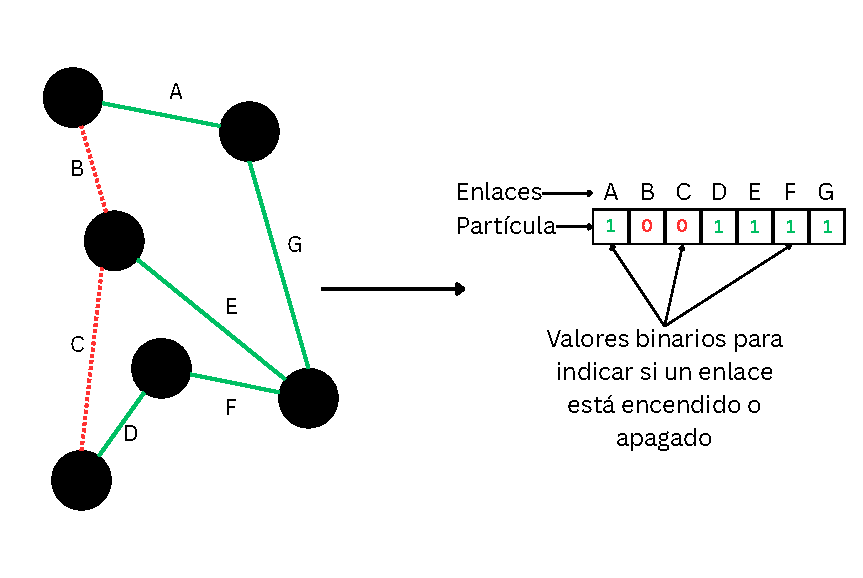
\includegraphics[width=0.6\textwidth]{pictures/pso_ejemplo.pdf}
\caption[Ejemplo sencillo PSO]{Representación de una red sencilla como partícula de PSO.\\Fuente: Elaboración propia.}
\label{fig:pso_ejemplo}
\end{figure}

La cantidad de partículas se ha establecido buscando un equilibrio entre la calidad de las soluciones encontradas y el tiempo de ejecución del algoritmo. Se han realizado varios barridos con la matriz de tráfico más cargada de la red Abilene, TM5, para averiguar cuál es el número más adecuado de partículas. Además, se aprovechó este mismo barrido para saber qué configuración de c1 y c2, coeficientes cognitivo y social, respectivamente, es la más eficiente. Los resultados que se obtuvieron en un primer momento son los que se pueden observar en la \autoref{fig:barrido_particulas_i1500}. Apenas hay que analizar la gráfica para darse cuenta de que los resultados son erráticos y poco concluyentes.

De manera intuitiva, se podría pensar que a medida que se incrementa el número de partículas, la calidad de las soluciones encontradas debería mejorar, ya que el algoritmo tiene más agentes explorando el espacio de búsqueda. Sin embargo, como puede observarse en la gráfica, no se aprecia una tendencia clara, sino que los resultados mejoran y empeoran a medida que se incrementa la cantidad de partículas.

\begin{figure}[H]
\centering
\captionsetup{justification=centering}
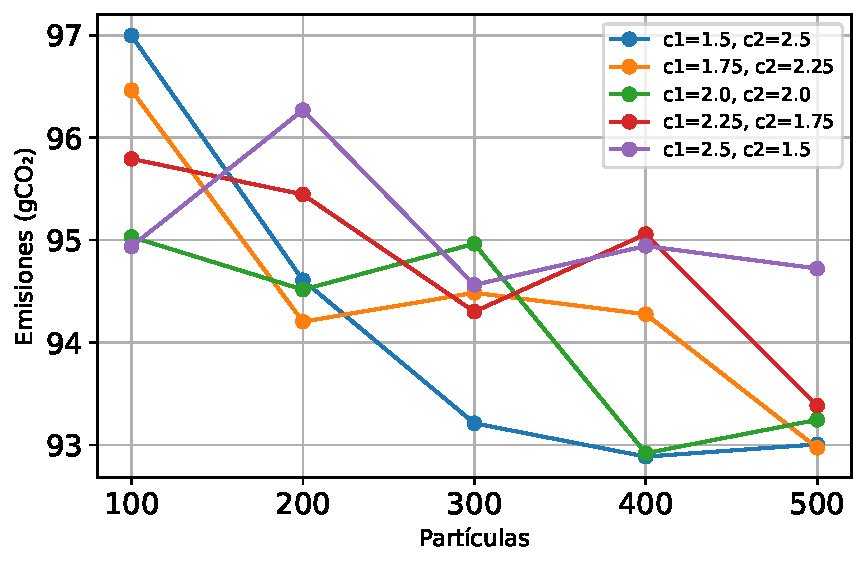
\includegraphics[width=0.6\textwidth]{pictures/i1500_particles_100-500.pdf}
\caption[Barrido partículas Abilene]{Resultados del barrido de partículas para la TM5 de Abilene. Iteraciones fijas en 1500.\\Fuente: Elaboración propia.}
\label{fig:barrido_particulas_i1500}
\end{figure}

Tras estos primeros resultados, se decidió investigar el por qué de los mismos. Tras la realización de diferentes pruebas, las cuales se comentarán con detalle más adelante en el \autoref{chp:results}, se descubrió un factor que estaba afectando a los resultados de manera significativa: la aleatoriedad con la que se incializan las partículas. Dado que PSO es un algoritmo estocástico, la inicialización aleatoria de las partículas puede llevar a resultados muy diferentes en cada ejecución, lo que explica la falta de una tendencia clara en los resultados del barrido. Para abordar este problema, se decidió inicializar las partículas de dos maneras: una de las partículas del enjambre se inicializa con todos los enlaces encendidos y el resto de partículas se inicializan con un porcentaje de enlaces encendidos que se comprende entre el 50\% y el 90\%.

En la \autoref{fig:barrido_particulas_i1500_inicializacion} se pueden observar los resultados del barrido de partículas con esta nueva estrategia de inicialización. En la gráfica se aprecia una clara tendencia a mejorar los resultados a medida que se incrementa el número de partículas, lo que confirma las sospechas sobre la influencia de la aleatoriedad en los resultados anteriores. Aunque todavía hay algún que otro pico, estos son despreciables en comparación con la mejora obtenida, pues disminuyen las emisiones entre 8 y 10 $gCO_2$.

\begin{figure}[H]
\centering
\captionsetup{justification=centering}
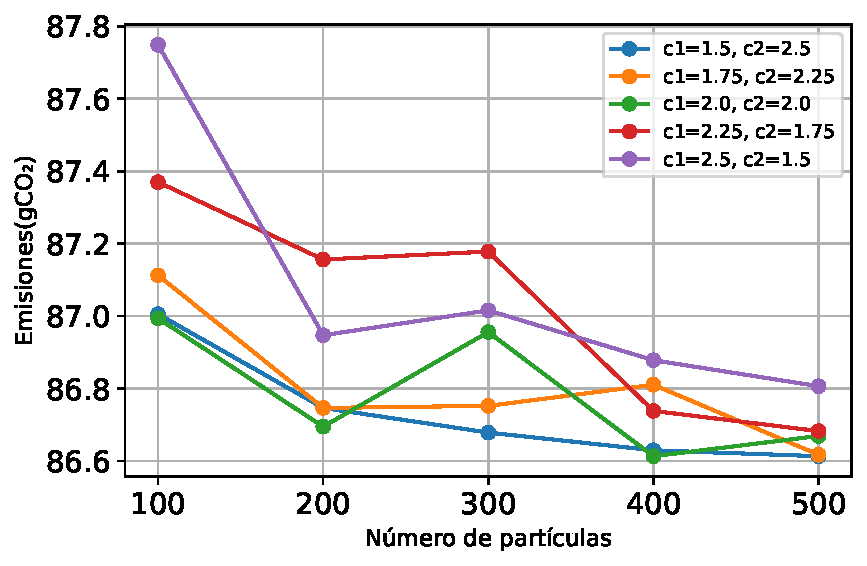
\includegraphics[width=0.6\textwidth]{pictures/particulas_100-500_i1500_v2.pdf}
\caption[Barrido partículas Abilene con inicialización controlada]{Resultados del barrido de partículas para la TM5 de Abilene con inicialización controlada de partículas. Iteraciones fijas en 1500.\\Fuente: Elaboración propia.}
\label{fig:barrido_particulas_i1500_inicializacion}
\end{figure}

Finalmente, se decidió usar 100 y 200 partículas para las pruebas finales. Por un lado, a partir de 200 partículas, las mejoras obtenidas no justificaban el incremento en el tiempo de ejecución. Por otro lado, aunque los resultados obtenidos con 100 partículas son ligeramente peores, la diferencia en el tiempo de ejecución es lo suficientemente alta como para justificar el uso de 100 partículas.

\subsection{Iteraciones}\label{sec:iteraciones}

Otro de los parámetros clave de PSO es el número de iteraciones, que determina cuántas veces las partículas tendrán que relizar el proceso de evaluación y actualización de sus posiciones. En general, un mayor número de iteraciones puede permitir que el algoritmo explore el espacio de búsqueda de manera más exhaustiva y encontrar mejores soluciones, pero también puede aumentar significativamente el tiempo de ejecución. Análogamente a lo que se hizo con las partículas, se realizaron dos barridos sobre la matriz TM5 de Abilene para averiguar cuál es el número de iteraciones más adecuado. Ambos barridos se realizaron desde 100 iteraciones hasta 1500, incrementando de 100 en 100, dejando fijas las partículas en 100 y 200, además de usar la misma estrategia de inicialización. También se aprovecharon estos barridos para averiguar qué configuración de c1 y c2 es la más eficiente.

\begin{figure}[H]
    \centering
    \captionsetup{justification=centering}
    \begin{subfigure}{0.48\textwidth}
        \captionsetup{justification=centering}
        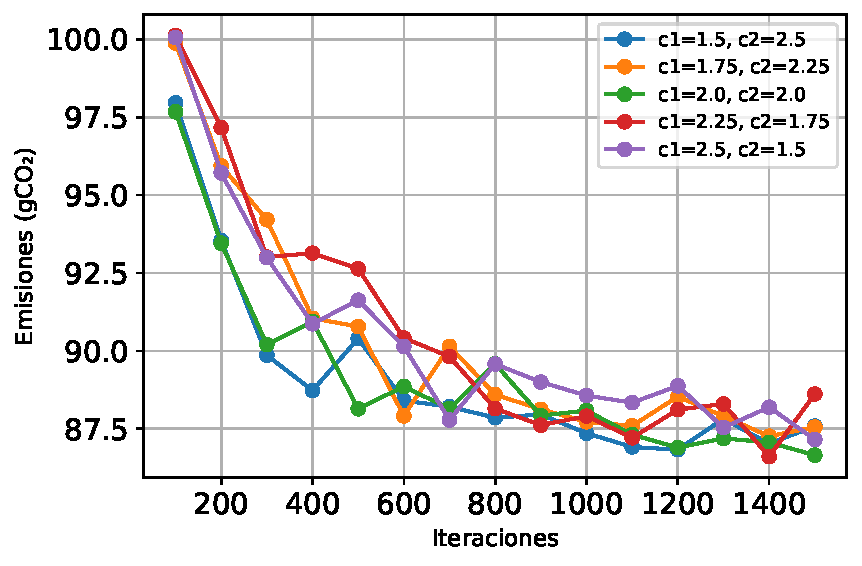
\includegraphics[width=\textwidth]{pictures/barrido_iters_100-1500_p100.pdf}
        \caption[Barrido iteraciones Abilene con 100 partículas]{Barrido con partículas fijas en 100.\\Fuente: Elaboración propia.}
        \label{fig:barrido_iters_p100}
    \end{subfigure}
    \hfill
    \begin{subfigure}{0.48\textwidth}
        \captionsetup{justification=centering}
        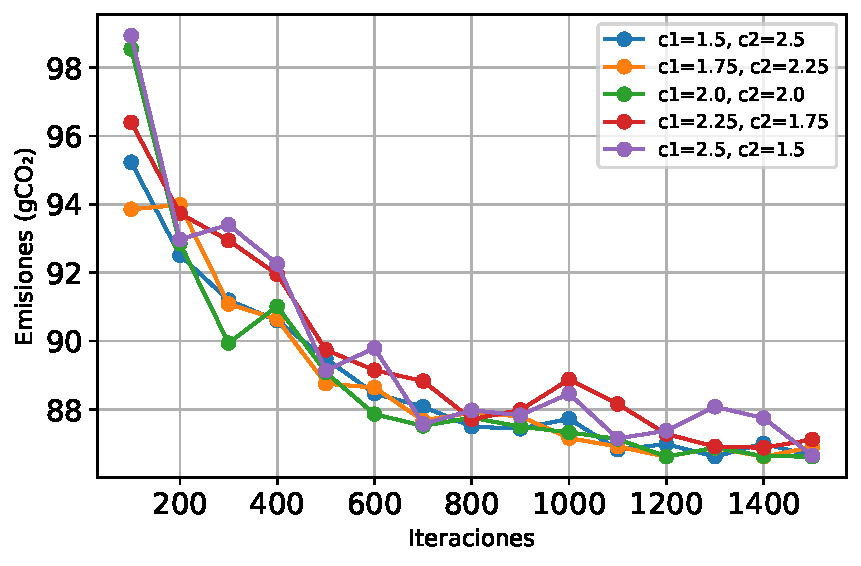
\includegraphics[width=\textwidth]{pictures/barrido_iters_100-1500_p200.pdf}
        \caption[Barrido iteraciones Abilene con 200 partículas]{Barrido con partículas fijas en 200.\\Fuente: Elaboración propia.}
        \label{fig:barrido_iters_p200}
    \end{subfigure}
    \caption[Barridos iteraciones Abilene]{Resultados de los barridos de iteraciones para la TM5 de Abilene con 100 y 200 partículas.}
    \label{fig:barridos_iters_100-1500}
\end{figure}

En los barridos mostrados en la \autoref{fig:barridos_iters_100-1500} se aprecia una clara tendencia a mejorar los resultados a medida que aumentan las iteraciones. En ambos casos, se observa que a partir de 600 iteraciones las mejoras que se obtienen son casi despreciables, por lo que se decidió fijar en 600 las iteraciones para las pruebas finales. De todas maneras, se decidió usar también 1200 iteraciones para comprobar si esta segunda configuración obtenía mejores resultados en escenarios más complejos, como pueden ser redes más grandes y con más tráfico.

Estas gráficas aportan información muy interesante sobre la influencia de las partículas en los resultados. En la \autoref{fig:barrido_iters_p100}, aunque todas las configuraciones de c1 y c2 mejoran los resultados al aumentar las iteraciones, se observa cierta disparidad entre las diferentes configuraciones. En cambio, en la \autoref{fig:barrido_iters_p200}, hay una mayor convergencia en los resultados obtenidos con las diferentes combinaciones de c1 y c2, lo que refuerza la decisión de usar 100 y 200 partículas para las pruebas finales.

\subsection{Coeficientes cognitivo y social}

Para determinar la configuración más adecuada de los coeficientes cognitivo y social, se aprovecharon los barridos realizados en las Subsecciones \ref{sec:conf_particulas} y \ref{sec:iteraciones}. En todos los barridos realizados, las configuraciones que ofrecían los mejores resultados eran aquellas en las que el coeficiente social era mayor que el cognitivo, es decir, aquellas en las que las partículas se centraban más en la explotación que en la exploración. Concretamente, las dos mejores configuraciones era $c_1 = 1.5$ y $c_2 = 2.5$ (gráfica azul) y $c_1 = 1.75$ y $c_2 = 2.25$ (gráfica naranja). Puesto que desde un principio se quería buscar que el algoritmo se centrase más en la explotación, se terminó optando por la gráfica naranja, es decir, por la configuración $c_1 = 1.75$ y $c_2 = 2.25$, pues ofrece un buen equilibrio entre la exploración personal y la explotación colectiva, dando cierta prioridad a esta última.

\subsection{Inercia, vecinos y dimensiones del espacio de búsqueda}

Un valor coherente para que el coeficiente de inercia, representado por $w$, fomente que las partículas se centren más en la explotación que en la exploración, pero sin dejar de lado esta última, es 0.7. Lo que indica este valor es que para la siguiente iteración, a la hora de actualizar la velocidad, se tendrá en cuenta en un 70\% la velocidad de la iteración anterior. Esto permite a las partículas explotar los resultados grupales a buen ritmo pero deja margen de maniobra en caso de que estos resultados no terminen de ser fructíferos.

En el caso del número de vecinos, la cantidad fijada para todas las pruebas ha sido 100. Esto permite tener dos escenarios durante los experimentos: cuando el enjambre se componga de 100 partículas, cada una tendrá acceso a la información de todo el enjambre; cuando sea de 200, cada agente solo considerará la mitad. Estos dos escenarios son muy interesantes, ya que el primero favorece una rápida convergencia hacia la solución global, mientras que el segundo fomenta más la exploración.

Por último, las dimensiones del espacio de búsqueda dependen por completo de la topología de red, puesto que es el número de enlaces unidireccionales de la red lo que las define. Esto se debe a que cada partícula representa una solución candidata en la que se asigna un estado a cada enlace, por lo que el número de variables de dicha solución coincide directamente con el número de enlaces de la red. Por lo tanto, redes con mayor número de enlaces darán lugar a espacios de búsqueda más grandes, incrementando así la complejidad del problema.

\subsection{Función objetivo y pseudocódigo}

Para modelar la función que usará el algoritmo de PSO para evaluar la calidad de las posibles soluciones, se parte de la fórmula propuesta en el artículo \textit{Exploring the Benefits of Carbon-Aware Routing} \cite{ElZahr2023}:

\begin{equation}
    C_{tot}(G, X, \lambda, c, \beta) = \sum_{n=1}^{V} (x_n * \lambda_n * c_n) + \sum_{l=1}^{E} \beta_l (c_{l_{n_1}} + c_{l_{n_2}})
\end{equation}

Donde:

\begin{itemize}
    \item $G$ es la topología de la red, representada como un grafo.
    \item $V$ y $E$ son el número de nodos y enlaces de la red, respectivamente.
    \item $x_n$ es la intensidad de flujo en el nodo $n$.
    \item $c_n$ es la tasa de emisiones de $CO_2$ asociada al nodo $n$.
    \item $\lambda_n$ es la potencia dinámica incremental por tasa de datos del nodo $n$.
    \item $\beta_l$ es el incremento del consumo de energía al habilitar un puerto.
    \item $c_{l_{n_1}}$ y $c_{l_{n_2}}$ son las emisiones de $CO_2$ asociadas a los nodos $n_1$ y $n_2$ que están conectados por el enlace $l$.
\end{itemize}

El primer sumatorio representa el consumo dinámico de energía asociado al tráfico que pasa por cada nodo, es decir, cuanto más tráfico pase por un nodo, más energía consumirá ese nodo. El segundo sumatorio se corresponde con el consumo estático de energía asociado a los enlaces que están activos. Un enlace activo implica que hay un puerto habilitado en cada uno de los nodos que conecta, lo que genera un consumo de energía adicional. La \autoref{fig:consumo_router} representa gráficamente lo que se acaba de explicar: la potencia estática es el consumo base de energía de un router y no se puede reducir. La potencia de los puertos es la cantidad de energía extra que se consume al habilitar un puerto. Este valor es orientativo, ya que el consumo real también depende del modo de operación en el que trabaje el router, puesto que cada modo influye en aspectos como la velocidad de los datos. Por último, la componente azul del modelo es la potencia dinámica, que depende de la carga de tráfico del router.

\begin{figure}[H]
\centering
\captionsetup{justification=centering}
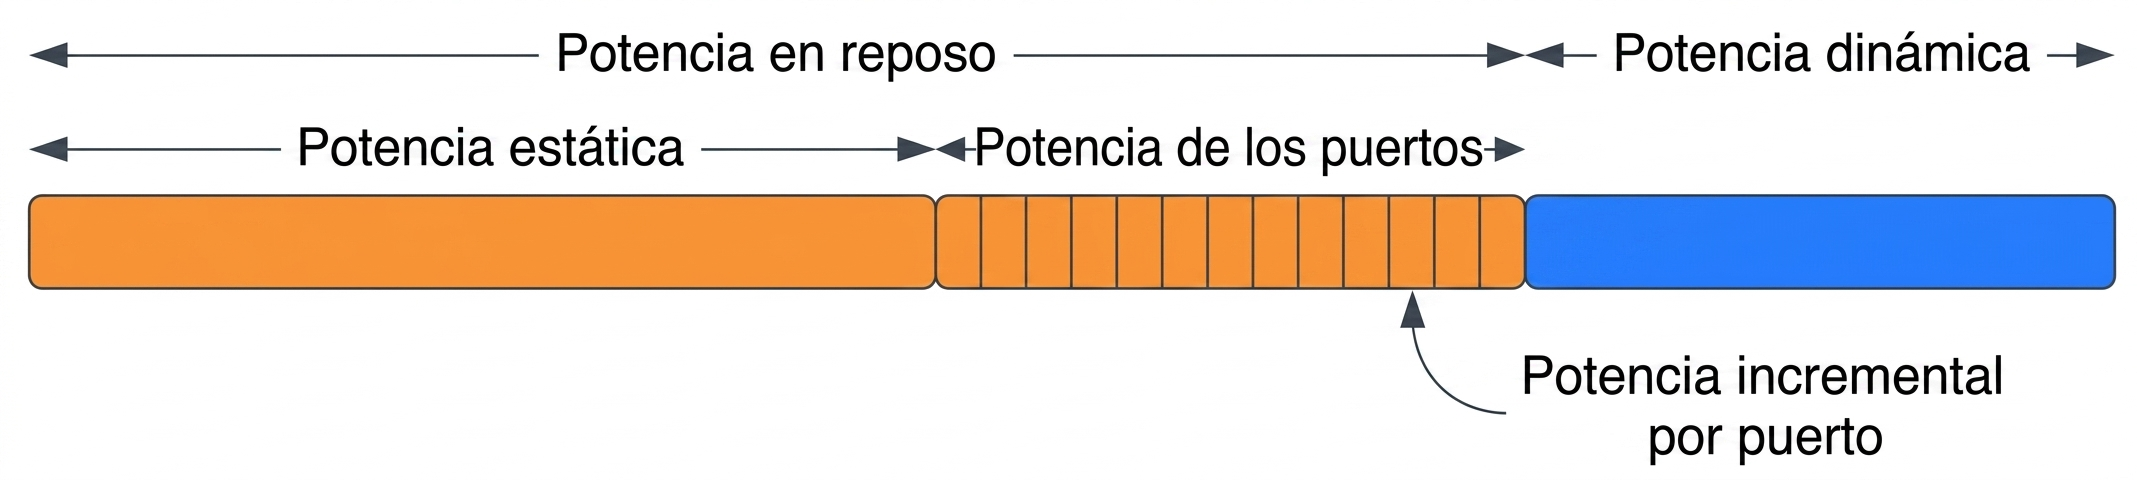
\includegraphics[width=0.7\textwidth]{pictures/consumo_router.png}
\caption[Esquema consumo router]{Modelo de consumo de energía de un router.\\Fuente: José Antonio Gómez de la Hiz \cite{GomezdelaHiz2025}.}
\label{fig:consumo_router}
\end{figure}

A lo largo de este trabajo, se ha mencionado en varias ocasiones la importancia de no dejar sin conexión ninguna parte de la red. Si a eso se le junta querer reducir la carga de nodos y enlaces en zonas de altas emisiones, se genera la necesidad de buscar los caminos que cumplan ambos requisitos, necesidad que puede satisfacerse con la estrategia \textit{K-Shortest Path} (KSP). Esta técnica permite encontrar los \textit{K} caminos más cortos entre dos puntos, aunque en este caso los caminos no son los más cortos sino los más eficientes, ambientalmente hablando. De esta manera, si la ruta que menos emisiones genera no tiene capacidad de enrutar todo el tráfico, se evaluaría la siguiente ruta.

Una vez explicada en detalle la fórmula en la que se basa la función objetivo, se procede a presentar el psudocódigo de la versión para PSO normal. El Algoritmo \ref{alg:carbon_pso}, dada una matriz de tráfico, asigna cada flujo al mejor camino disponible, procesando primero las demandas más grandes. Un camino se considera válido si solamente utiliza enlaces activos de la red y dispone de capacidad suficiente para satisfacer la demanda. Si algún flujo no puede ser asignado, la solución se considera inválida y se devuelve $+\infty$. Una vez asignados todos los flujos, se calcula la emisión de carbono tal y como se ha explicado con anterioridad: la potencia dinámica $P_{\text{dyn}}$, proporcional al tráfico en cada nodo, y la potencia de los puertos $P_{\text{ports}}$, asociada a los enlaces activos de la topología. Las emisiones totales de carbono de la red es el resultado de sumar ambos términos.

\begin{algorithm}[H]
    \caption{Cálculo de la emisiones totales de la red para PSO normal}
    \label{alg:carbon_pso}
    \begin{algorithmic}[1]
    \Require $\text{position}[N][N]$, $\text{flow\_matrix}[N][N]$, $\text{all\_k\_paths}$, $\text{nodes\_max\_flow}[N][N]$, $\text{carbon\_intensity}[N]$
    \Ensure Emisiones totales de carbono de la red
    
    \State Inicializar $\text{nodes\_traffic} \leftarrow 0$, $\text{links\_traffic} \leftarrow 0$, $P_{\text{dyn}} \leftarrow 0$, $P_{\text{ports}} \leftarrow 0$
    \State $\mathcal{A} \leftarrow \{(i,j) \mid \text{position}[i][j] = 1\}$
    
    \State Ordenar demandas $\mathcal{D}$ de forma descendente por $\text{flow\_matrix}[s][d]$
    
    \For{$(s, d, \delta) \in \mathcal{D}$}
        \State $p^* \leftarrow$ primer camino en $\text{all\_k\_paths}[(s,d)]$ válido y con capacidad $\geq \delta$
        \If{$p^* = \textsc{None}$} \Return $+\infty$ \EndIf
        \State Actualizar $\text{links\_traffic}$ y $\text{nodes\_traffic}$ según $p^*$ y $\delta$
    \EndFor
    
    \For{$x \leftarrow 0$ \textbf{ to } $N-1$}
        \State $c_x \leftarrow \text{carbon\_intensity}[x] / 1000$
        \State $P_{\text{dyn}} \mathrel{+}= \text{nodes\_traffic}[x] \cdot \lambda_n \cdot c_x$
        \For{$y \neq x$ \textbf{ con } $\text{position}[x][y] \neq 0$}
            \State $P_{\text{ports}} \mathrel{+}= \beta_l \cdot (c_x + c_y)$
        \EndFor
    \EndFor
    
    \State \Return $P_{\text{dyn}} + P_{\text{ports}}$
    \end{algorithmic}
\end{algorithm}

A continuación se presenta la variante del algoritmo anterior que introduce el mecanismo de penalización VCH. Cuando un flujo no puede ser asignado por ausencia de un camino válido o falta de capacidad, el Algoritmo \ref{alg:carbon_vch} lo cuenta como una violación. Al finalizar la asignación, el número de violaciones se multiplica por un factor de penalización $M$ y se añade a las emisiones de carbono. Esto permite que el algoritmo siempre devuelva un valor finito, penalizando las soluciones que incumplen las restricciones de la red.

\begin{algorithm}[H]
\caption{Cálculo de la emisiones totales de la red para PSO VCH}
\label{alg:carbon_vch}
\begin{algorithmic}[1]
\Require $\text{position}[N][N]$, $\text{flow\_matrix}[N][N]$, $\text{all\_k\_paths}$, $\text{nodes\_max\_flow}[N][N]$, $\text{carbon\_intensity}[N]$, $M$
\Ensure Intensidad de carbono total de la red, penalizada por violaciones

\State Inicializar $\text{nodes\_traffic} \leftarrow 0$, $\text{links\_traffic} \leftarrow 0$, $P_{\text{dyn}} \leftarrow 0$, $P_{\text{ports}} \leftarrow 0$, $v \leftarrow 0$
\State $\mathcal{A} \leftarrow \{(i,j) \mid \text{position}[i][j] = 1\}$
\State Ordenar demandas $\mathcal{D}$ de forma descendente por $\text{flow\_matrix}[s][d]$

\For{$(s, d, \delta) \in \mathcal{D}$}
    \State $p^* \leftarrow$ primer camino en $\text{all\_k\_paths}[(s,d)]$ válido y con capacidad $\geq \delta$
    \If{$p^* = \textsc{None}$}
        \State $v \mathrel{+}= 1$ \Comment{Contabilizar violación y continuar}
    \Else
        \State Actualizar $\text{links\_traffic}$ y $\text{nodes\_traffic}$ según $p^*$ y $\delta$
    \EndIf
\EndFor

\For{$x \leftarrow 0$ \textbf{ to } $N-1$}
    \State $c_x \leftarrow \text{carbon\_intensity}[x] / 1000$
    \State $P_{\text{dyn}} \mathrel{+}= \text{nodes\_traffic}[x] \cdot \lambda_n \cdot c_x$
    \For{$y \neq x$ \textbf{ con } $\text{position}[x][y] \neq 0$}
        \State $P_{\text{ports}} \mathrel{+}= \beta_l \cdot (c_x + c_y)$
    \EndFor
\EndFor

\State \Return $P_{\text{dyn}} + P_{\text{ports}} + v \cdot M$
\end{algorithmic}
\end{algorithm}